\subsection{Energie}

\subsubsection{Recherchegrund}

Mit der Recherche über die Energie, können wir abschätzen wie viel Energie gewonnen werden kann und welche Turbine dafür geeignet ist.

\subsubsection{Ergebnisse}

\paragraph{Berechnung}

Um Energie aus fliessendem Wasser zu gewinnen gibt es drei unterschiedliche Möglichkeiten/Turbinen.  Diese wären das Wasserrad, die Gleichdruckturbine und die Überdruckturbine. Wir haben uns entschieden, dass eine Gleichdruckturbine, genauer eine Pelton-Turbine, für unsere Anwendung am besten geeignet ist.

\begin{center}
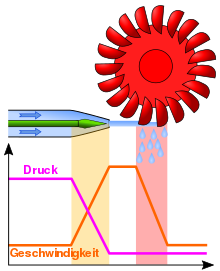
\includegraphics[width=5cm]{Gleichdruckturbine.png}
\end{center}

Das Wasser wird von einer gewissen Höhe in eine Fallleitung nach unten befördert. Die potenzielle Energie des Wassers wird dabei in kinetische Energie umgewandelt und das Wasser triff mit einer Geschwindigkeit unten aus. Um diese Energie zu nutzen wird der Wasserstrahl auf die Schaufeln der Pelton-Turbine gerichtet, die anschliessend zu drehen beginnt.
\newline
\newline 
\newline
Die Endgeschwindigkeit des Wassers kann mit folgender Formel berechnet werden:
\begin{center}
\(v = \sqrt{2 \cdot g \cdot h} \)
\end{center}

Die Einheit der Geschwindigkeit \(v\) ist \si{m/s}. Das Schwerefeld \(g\) auf der Erde besitzt den Wert 9.81~\si{N/Kg}. Und die Höhe \(h\) hat die Einheit \si{m}.
\newline 
\newline 
\newline
Die Energie die gewonnen werden kann, wird mit folgender Formel berrechnet:

\begin{center}
\(E =\frac 12\ \cdot m \cdot v^2\)
\end{center}

Die Energie  \(E\)  hat die Einheit  \si{J}. Die Einheit der Geschwindigkeit \(v\) ist \si{m/s} und die Masse \(m\) hat die Einheit \si{Kg}

\newpage

Um die Leistung zu erhalten, muss die Masse pro Zeit(1s) einberechnet werden. Die Masse wird  mit der Dichte und dem Volumenstrom ersetzt.

\begin{center}
\(P =\frac 12\ \cdot \varphi \cdot Q \cdot v^2\)
\end{center}

Die Leistung \(P\) hat die Einheit \si{W}. Der Volumentstrom \(Q\) hat die Einheit \si{m^3/s}. Die Einheit der Dichte \(\varphi\) ist \si{Kg/m^3} und die Einheit der Geschwindigkeit \(v\) ist \si{m/s}.
\newline 
\newline
 \newline


Mit diesen physikalischen Grundlagen kann nun die Leistung in Abhängigkeit der Höhe und des Volumenstromes berechnet werden. 

\begin{center}
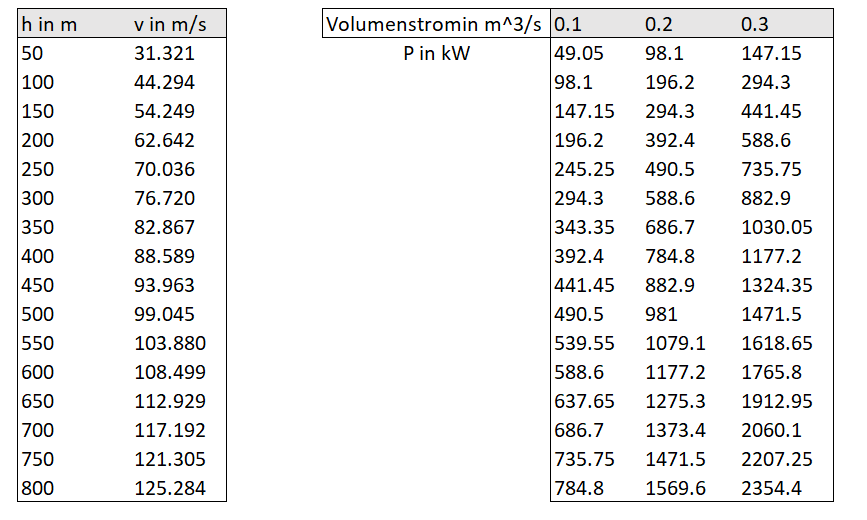
\includegraphics[width=10cm]{Leistungsberechnung.png}
\end{center}

Dies ist nur die Theoretische Leistung. Mit der Reibung am Rohr und dem Widerstand der Luftsäule wird das Wasser stark abgebrämst. Gemäss dem IZEG, die Versuche mit der Fallgeschwindigkeit durchgeführt haben, wird das Wasser bereichts nach 15m nicht mehr mehrklich schneller.

\begin{center}
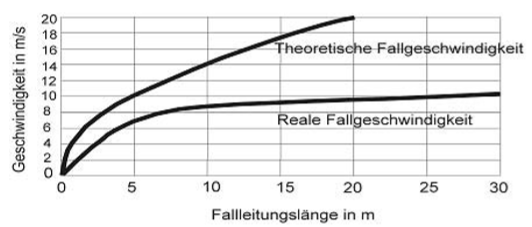
\includegraphics[width=10cm]{Fallgeschwindigkeit.png}
\end{center}

Mit der Endgeschwindigkeit von 10 \si{m/s}. wird bei einem Volumenstrom von 0.1 \si{m^3/s} noch 5 \si{kW} erzeugt.

\subsubsection{Fazit}

Die gewonnene Leistung nimmt ab ca. 15m nicht mehr merklich zu. Der Grundgedanke, dass die Geschwindigkeit des Wassers in grossen Fallhöhen zunimmt, funktioniert nur, wenn die Fallleitung komplett mit Wasser befüllt wäre und somit der Luftwiderstand wegfällt.

Damit man mit diesem System trotzem Energie zurückgewinnen kann, müsste all 15m eine Turbine die Energie des Wassers umwandeln.

\clearpage 





